\begin{frame}[fragile]
    \frametitle{Implémentation naïve de la multiplication de matrices}
    Principe:
    \[
        C_{ij} = \sum_{k=1}^{n} a_{ik}b_{kj}\quad\textrm{pour}\quad i = 1, \dots, m\quad \textrm{et}\quad j = 1,\dots,p
    \]\pause{}

    Pour exécuter il faut configurer créer le contexte d'exécution:\pause{}
    \begin{lstlisting}[language=Python]
    import pyopencl as cl
    # choose first platform 
    platform = cl.get_platforms()[0]       
    # retrieve platform devices to create context
    devices = platform.get_devices()        
    # create context for platform
    context = cl.Context(devices=devices)    
    # add OpenCL source code to context (source is a string)
    program_source = cl.Program(context, source)
    # compile the kernel
    program = program_source.build()
    # create the command queue for the context => make the builded programs avaiable for execution
    queue = cl.CommandQueue(context)
    \end{lstlisting}
\end{frame}

\begin{frame}[fragile]
    \frametitle{Implémentation naïve de la multiplication de matrices}
    Définition du kernel \textit{(program\_source)}:
    \begin{lstlisting}[language=c]
    __kernel void matrix_mult(__global float *a,
                              __global float* b,
                              __global float* c,
                              const unsigned int a_ncol,
                              const unsigned int b_ncol) {
        int rows = get_global_id(0);    /* iterate over rows */
        int columns = get_global_id(1); /* then iterate over columns */

        /* compute value */
        float value = 0;
        for (unsigned int i = 0 ; i < a_ncol ; i++) {
            value += a[rows * a_ncol + i] * b[i * b_ncol + columns];
        }

        c[rows * b_ncol + columns] = value;
    }
    \end{lstlisting} 
\end{frame}

\begin{frame}[fragile]
    \frametitle{Implémentation naïve de la multiplication de matrices}
    \begin{lstlisting}[language=python]
    import numpy as np
    import pyopencl as cl

    # a_dim is a tuple with (row, column) for A
    A = np.random.rand(A_dim[0] * A_dim[1]).astype(np.float32)   
    # b_dim ditto
    B = np.random.rand(B_dim[0] * B_dim[1]).astype(np.float32)   
    C = np.zeros(A_dim[1] * B_dim[0], dtype=np.float32)

    A_buffer = cl.Buffer(context, flags=cl.mem_flags.READ_ONLY, size=A.nbytes)
    B_buffer = cl.Buffer(context, flags=cl.mem_flags.READ_ONLY, size=B.nbytes)
    C_buffer = cl.Buffer(context, flags=cl.mem_flags.WRITE_ONLY, size=C.nbytes)

    cl.enqueue_copy(queue, src=A, dest=A_buffer)
    cl.enqueue_copy(queue, src=B, dest=B_buffer)

    kernel_arguments = (A_buffer, B_buffer, C_buffer, A_dim[1], B_dim[1])
    # .wait() to wait for the event to finish
    program.matrix_mult(queue, 
                       [A_dim[0], B_dim[1]],     # global dimensions
                       None, 
                       *kernel_arguments).wait()

    cl.enqueue_copy(queue, src=C_buffer, dest=C)
    \end{lstlisting}
\end{frame}

\begin{frame}
    \frametitle{Implémentation naïve de la multiplication de matrices}
    Trois genres de mesures:\pause{}
    \begin{itemize}
        \item le temps de copie des \textit{buffers}\pause{}
        \item le temps d'exécution\pause{}
        \item la précision des résultats\pause{}
    \end{itemize}\pause{}
    \vspace{20pt}
    Des matrices carrées de même dimension allant de 10 à 1 500 lignes/colonnes par pas de 10.
\end{frame}

\begin{frame}
    \frametitle{Implémentation naïve de la multiplication de matrices}
    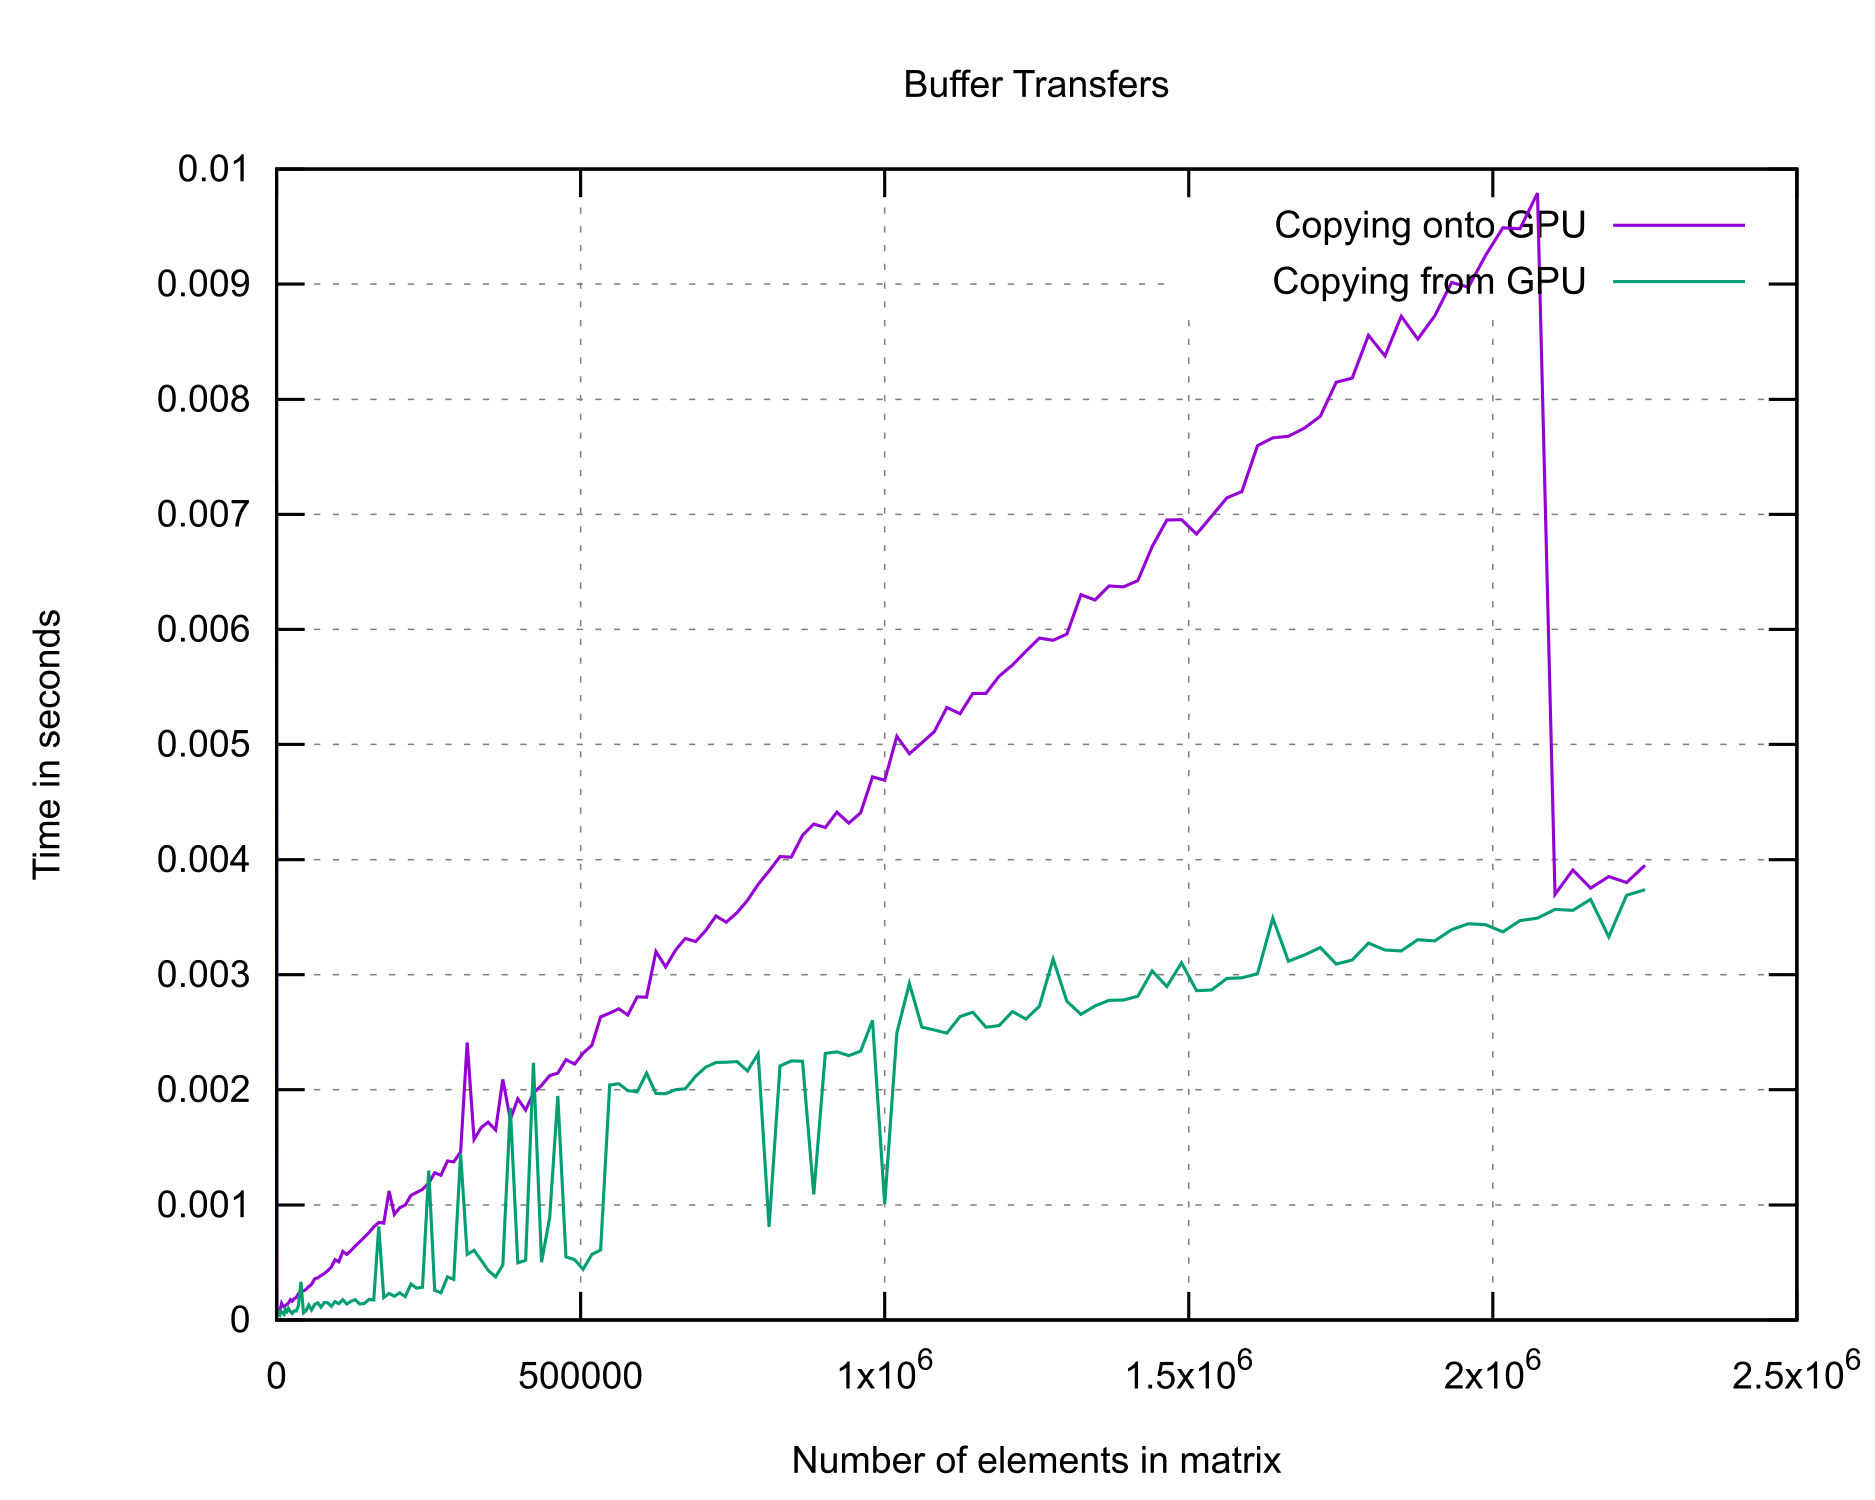
\includegraphics[width=\textwidth]{../resources/matrix_naive_buffer_transfer.png}
\end{frame}

\begin{frame}
    \frametitle{Implémentation naïve de la multiplication de matrices}
    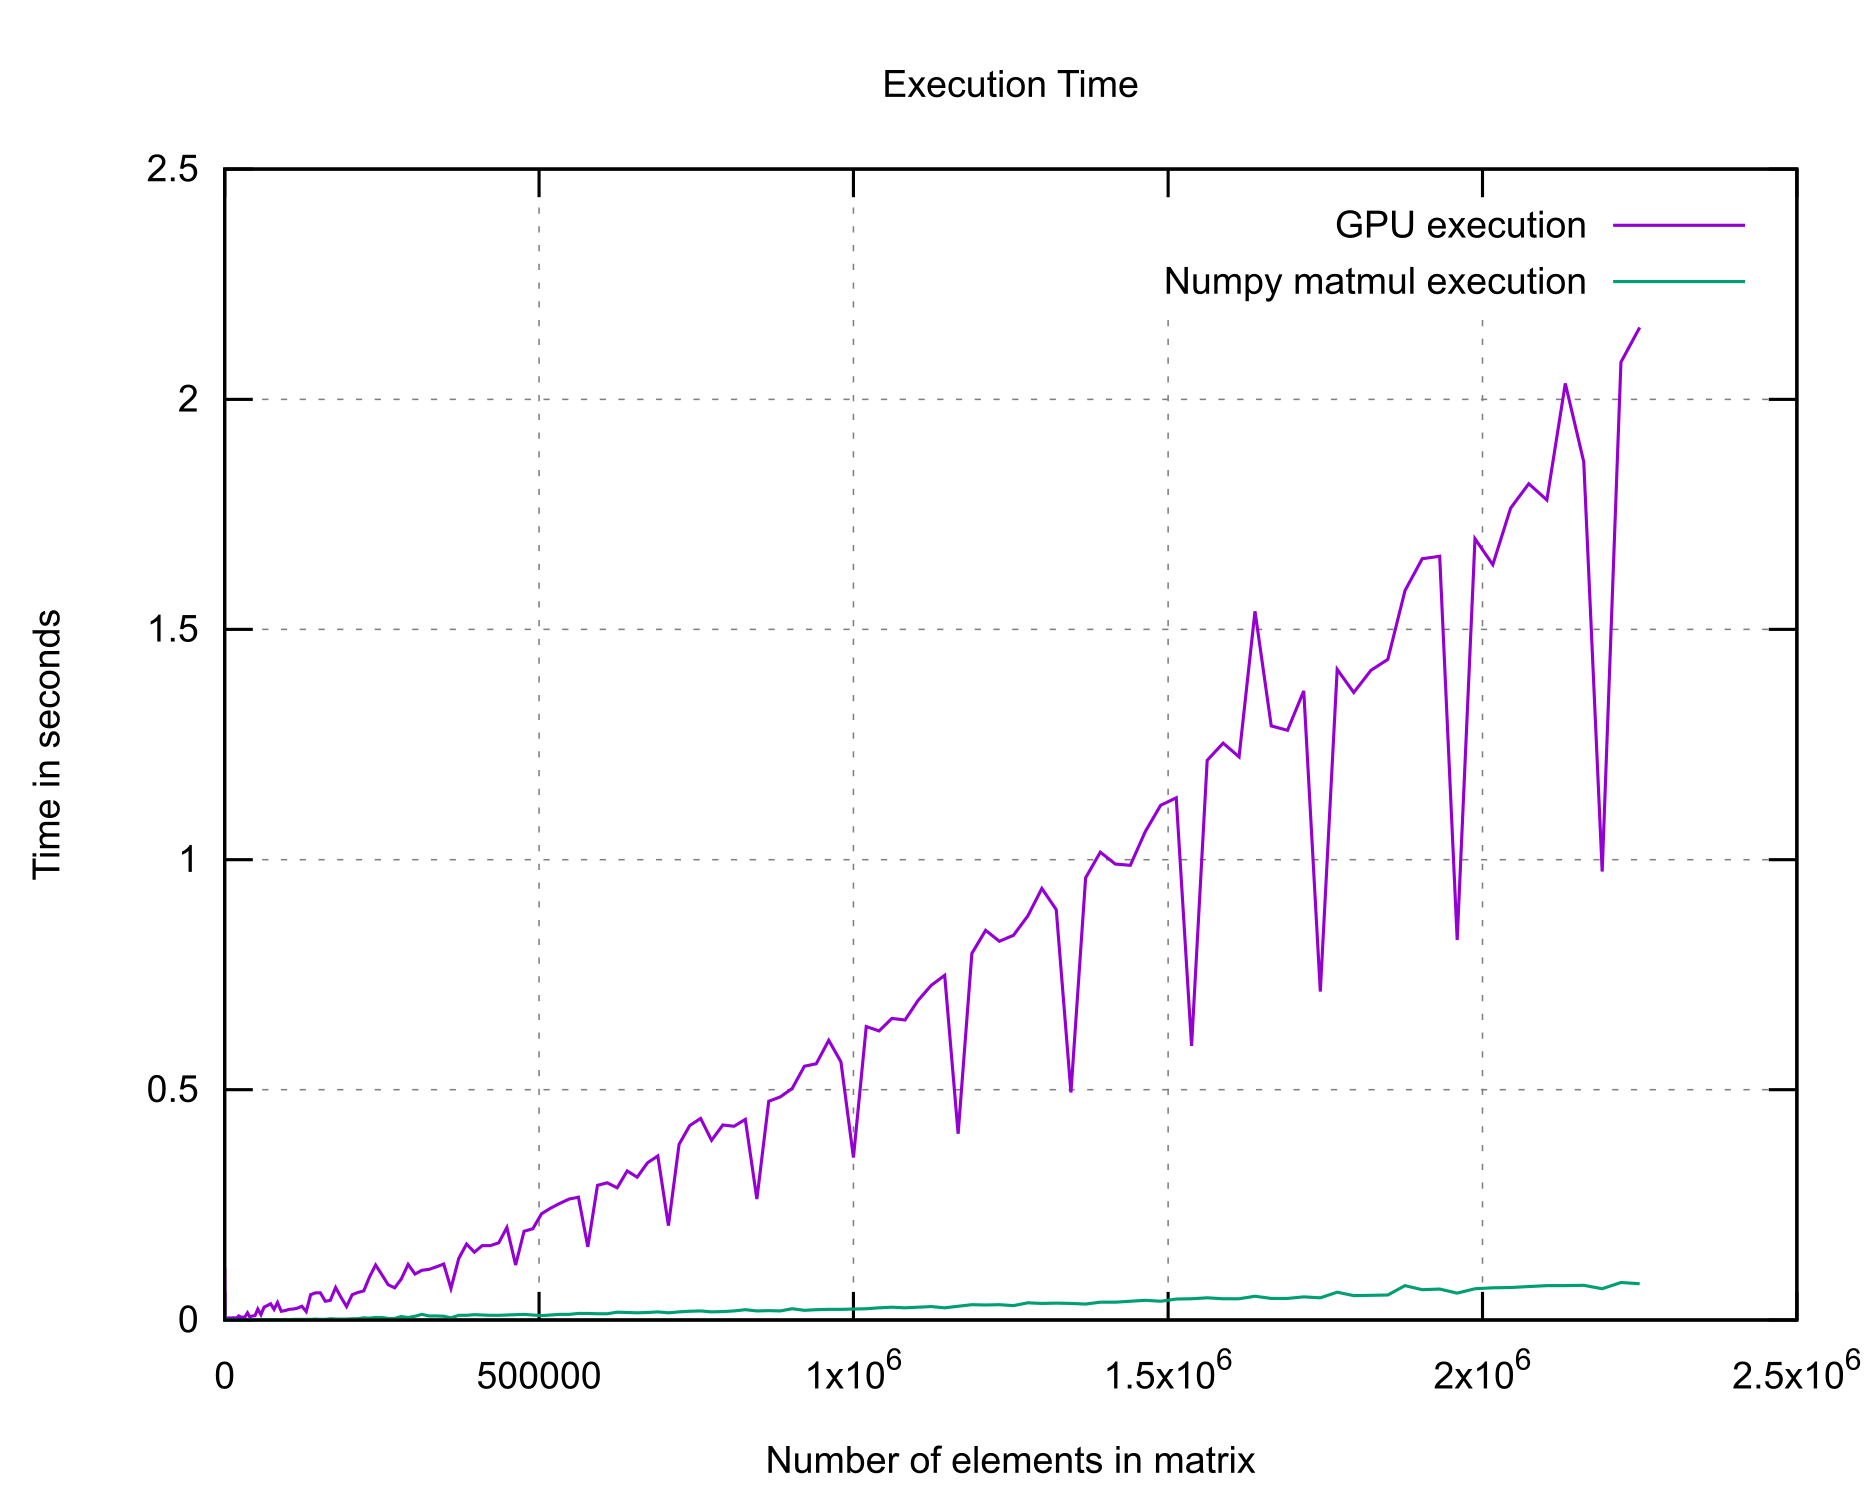
\includegraphics[width=\textwidth]{../resources/matrix_naive_execution_time.png}
\end{frame}

\begin{frame}
    \frametitle{Implémentation naïve de la multiplication de matrices}
    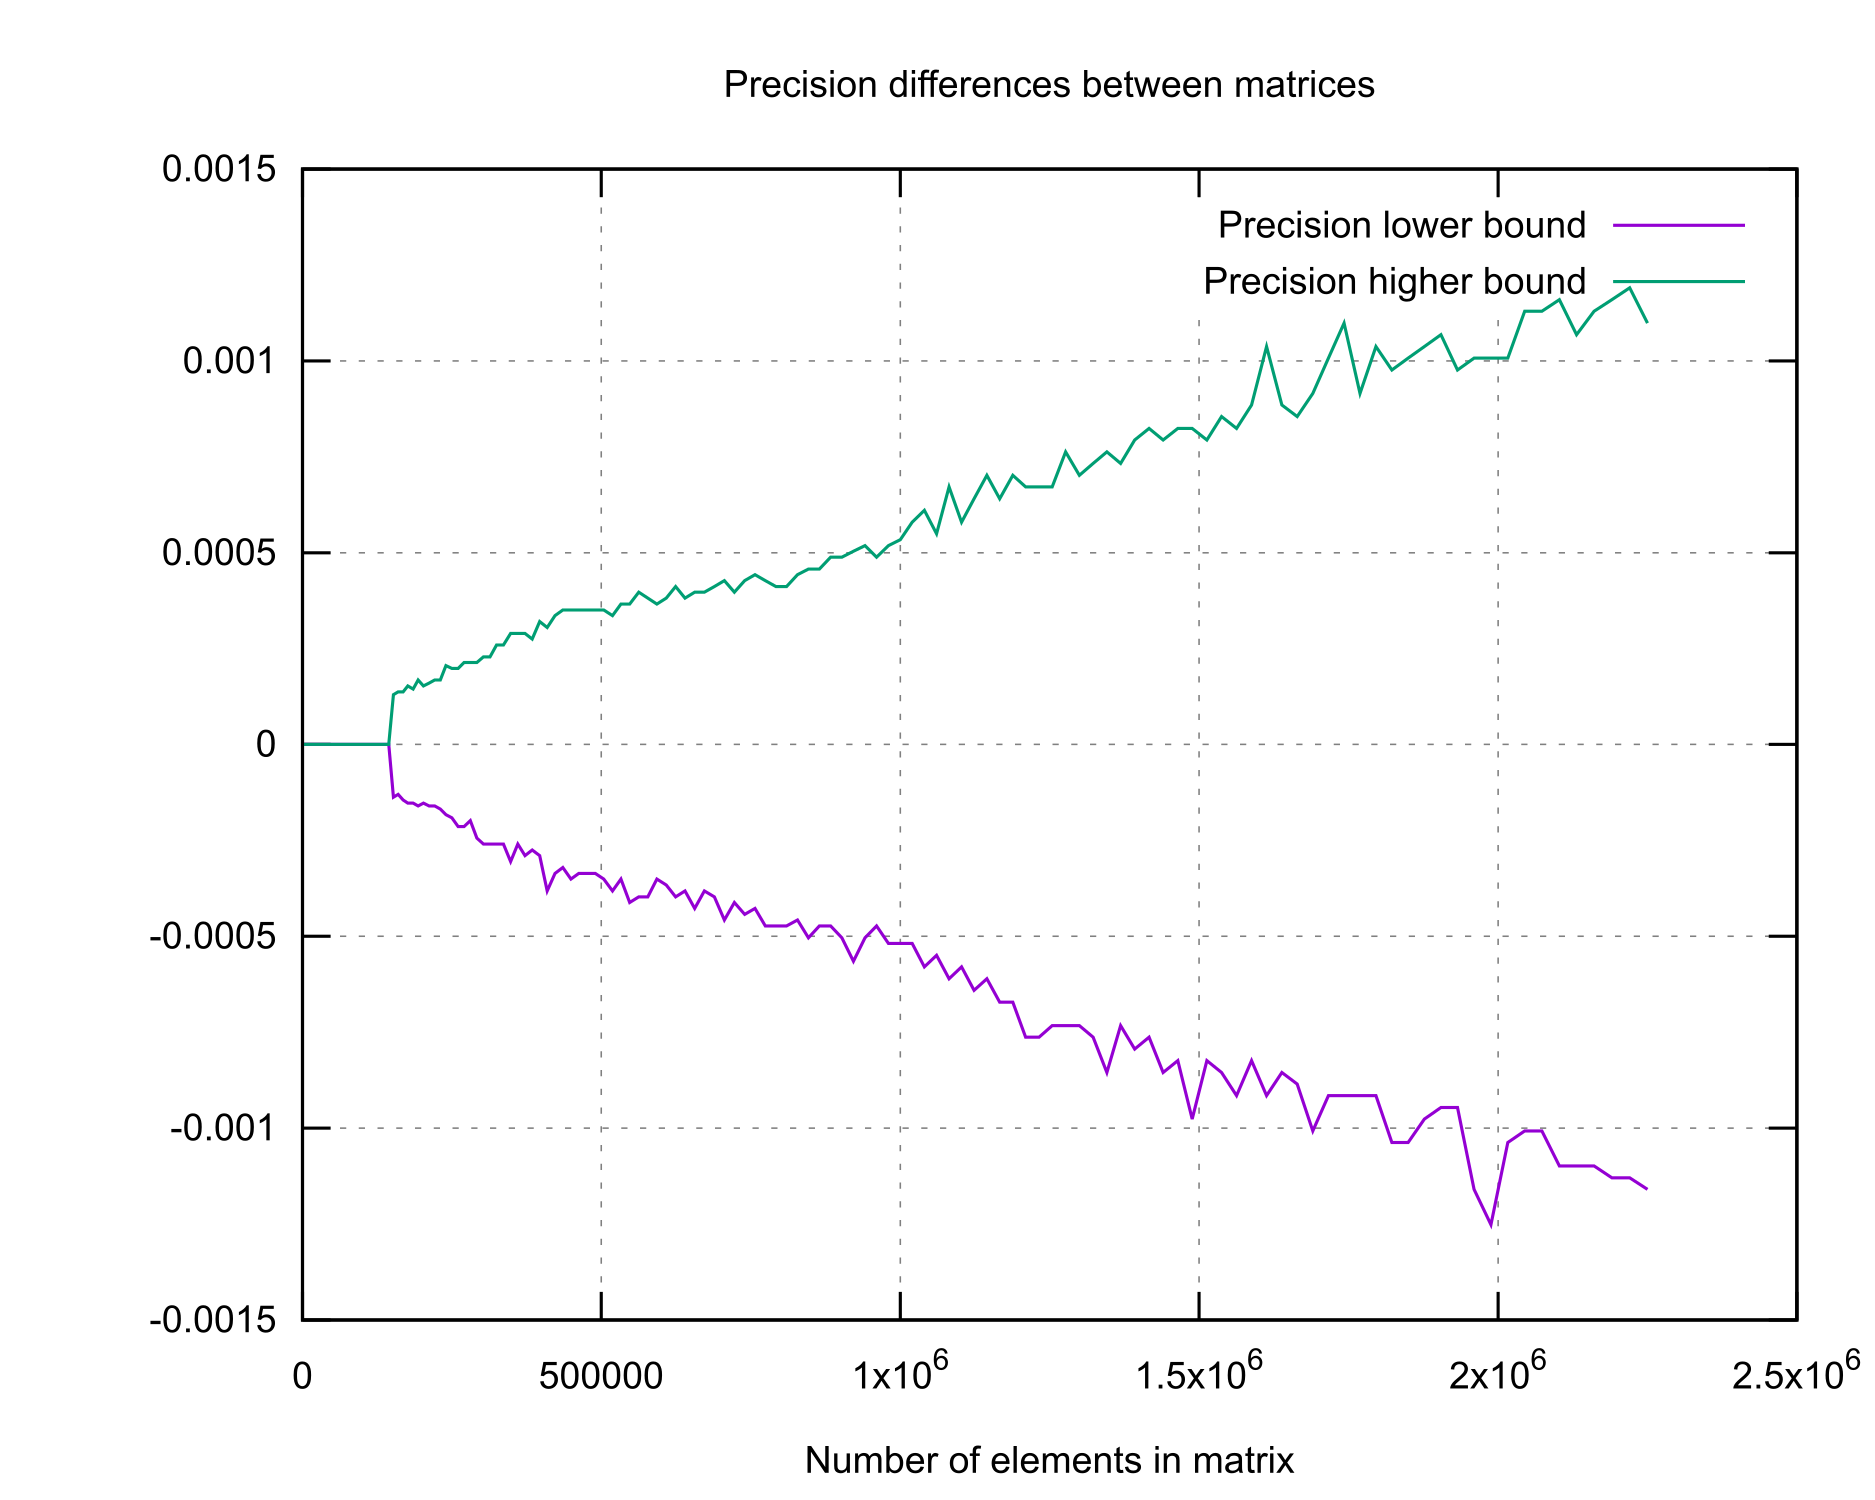
\includegraphics[width=\textwidth]{../resources/matrix_naive_float_precision.png}
\end{frame}

\begin{frame}
    \frametitle{Implémentation naïve de la multiplication de matrices}
    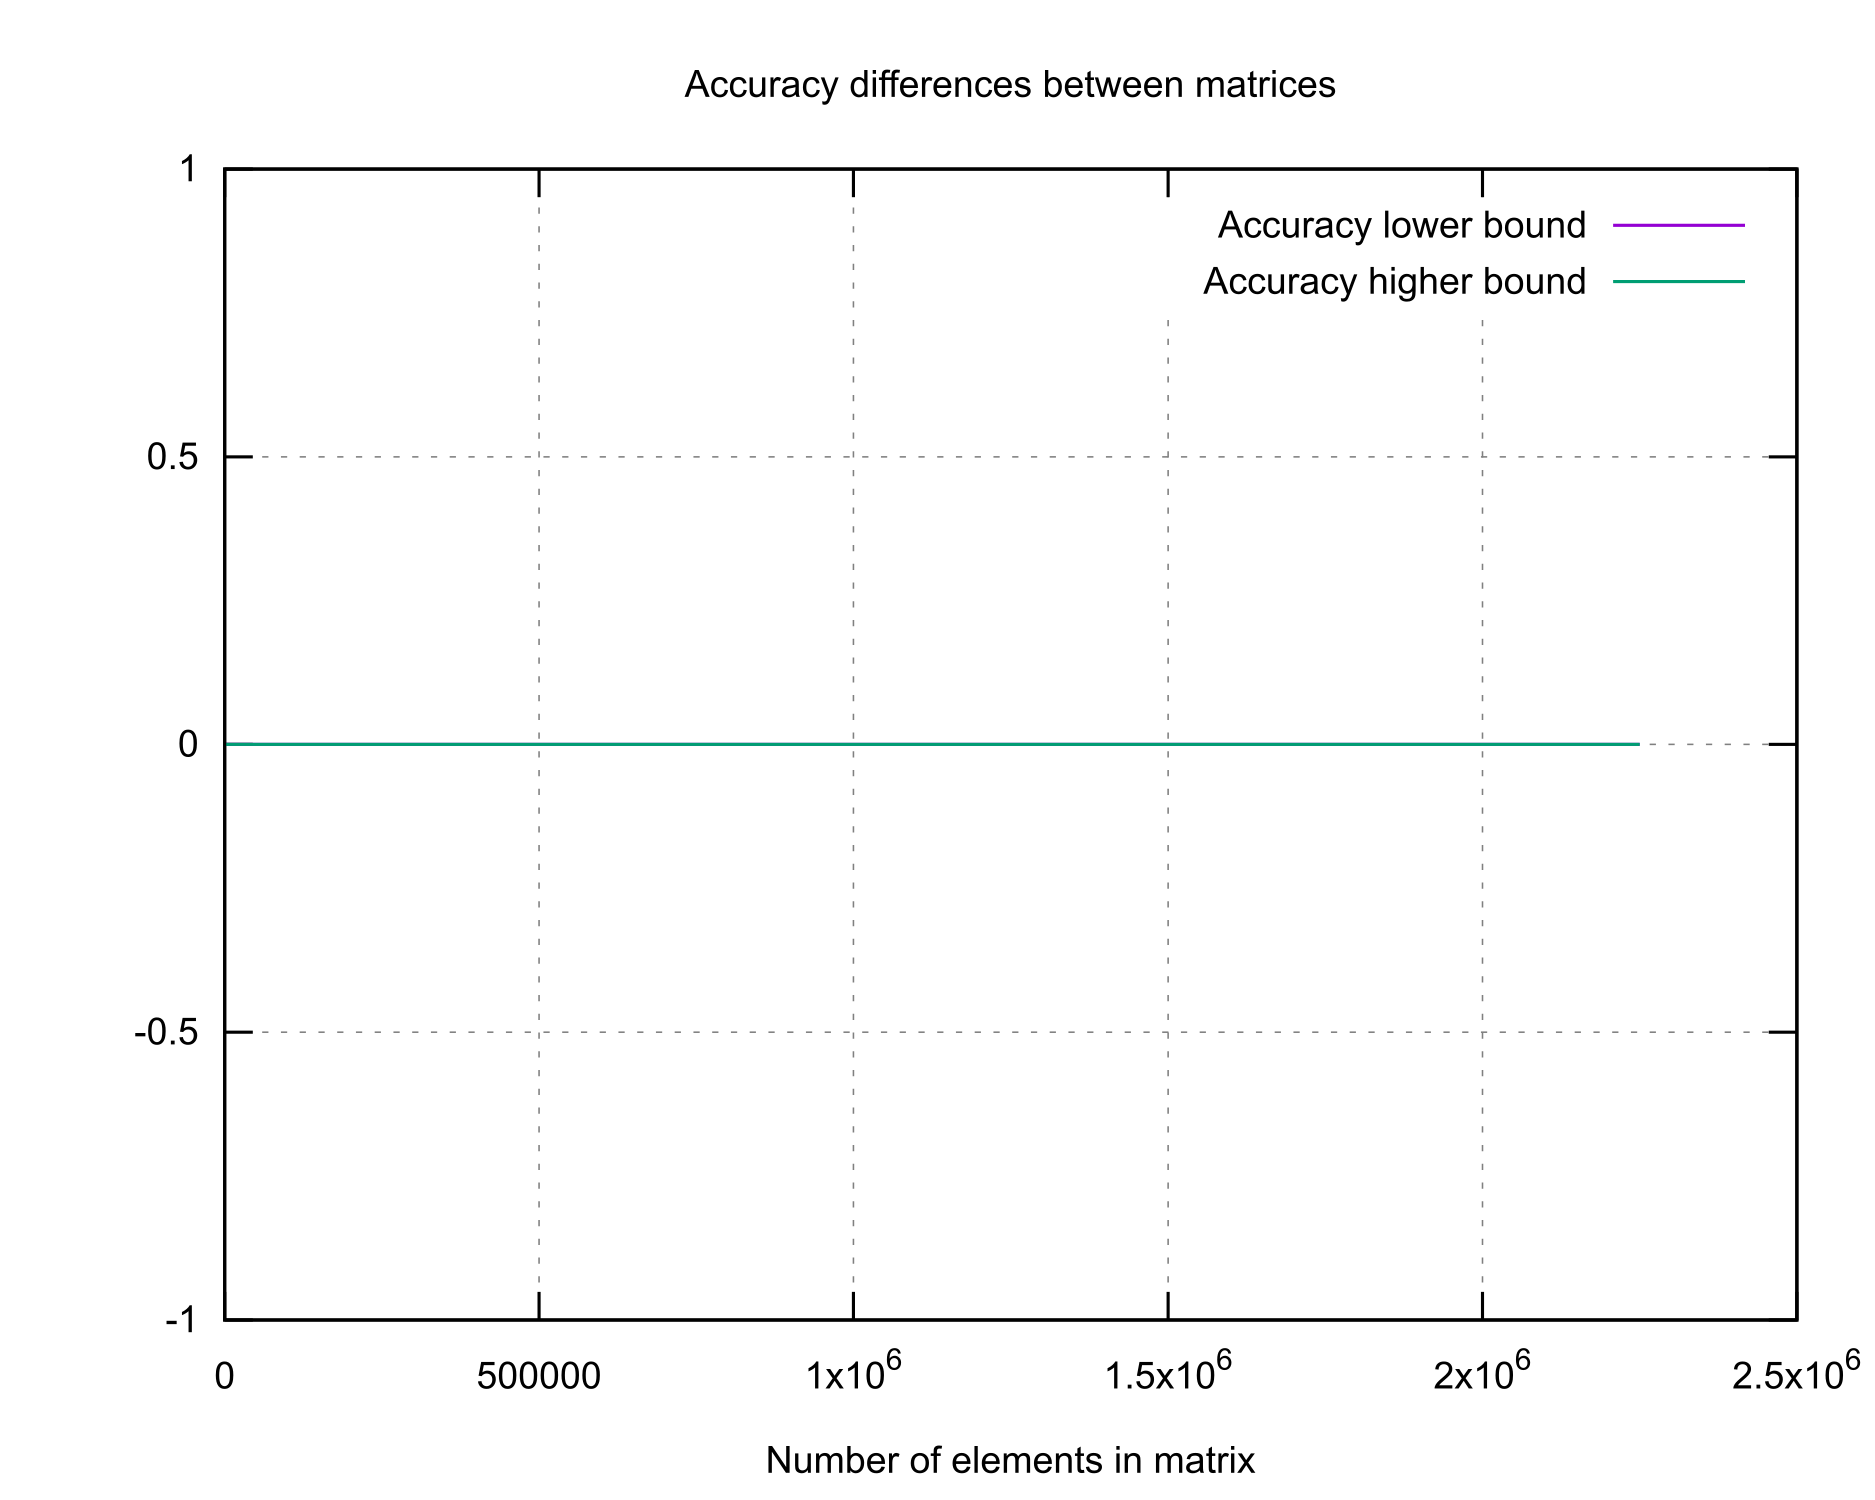
\includegraphics[width=\textwidth]{../resources/naive_integer_accuracy.png}
\end{frame}
